% ------------------------------------------------------------------------------
% TYPO3 CMS 6.2 LTS - What's New - Chapter "Backend Changes" (Serbian Version)
%
% @author	Sinisa Mitrovic <mitrovic.sinisaa@gmail.com>
% @license	Creative Commons BY-NC-SA 3.0
% @link		http://typo3.org/download/release-notes/whats-new/
% @language	Serbian
% ------------------------------------------------------------------------------
% Chapter: Backend Changes
% ------------------------------------------------------------------------------

\section{Promene administratorskog dela}
\section{Promene administratorskog dela}
\begin{frame}[fragile]
	\frametitle{Promene administratorskog dela}

	\begin{center}\huge{Poglavlje 3:}\end{center}
	\begin{center}\huge{\color{typo3darkgrey}\textbf{Promene administratorskog dela}}\end{center}

\end{frame}

% ------------------------------------------------------------------------------
% Autofocus
% ------------------------------------------------------------------------------
% http://forge.typo3.org/issues/49228

\begin{frame}[fragile]
	\frametitle{Promene administratorskog dela}
	\framesubtitle{Logovanje na administratorski deo}

 	\begin{itemize}
		\item Autofokus na korisnicko ime u formi za logovanje na administratorski deo\newline
			(HTML5 atribut: \texttt{autofocus="autofocus"})
	\end{itemize}

	\begin{figure}
		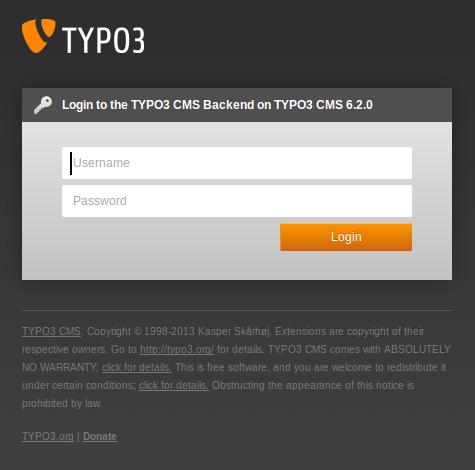
\includegraphics[width=0.4\linewidth]{Images/BackendChanges/BackendLogin.png}
	\end{figure}

\end{frame}

% ------------------------------------------------------------------------------
% Visual Appearance
% ------------------------------------------------------------------------------
% http://forge.typo3.org/issues/48376

\begin{frame}[fragile]
	\frametitle{Promene administratorskog dela}
	\framesubtitle{Vizualni prikaz}

	\begin{columns}[T]

		\begin{column}{.5\textwidth}
			\begin{itemize}
				\item Poboljsana upotrebljivost uz pomoc osvezenog layout-a
				\item Margine izmedju stavki modula (leva kolona) su povecane
				\item Baziran na mrezi od 12 piksela, koji je udvostucen
			\end{itemize}

			\advance\leftskip+3.8cm

			\smaller
				Levo: TYPO3 4.5\newline
				Desno: TYPO3 6.2
			\normalsize
		\end{column}

		\begin{column}{.5\textwidth}
			\begin{figure}\vspace*{-0.4cm}
				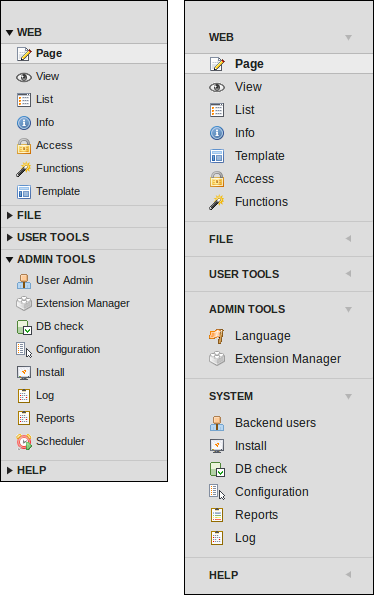
\includegraphics[width=0.6\linewidth]{Images/BackendChanges/VisualAppearance.png}
			\end{figure}
		\end{column}

	\end{columns}

\end{frame}

% ------------------------------------------------------------------------------
% Visual Appearance
% ------------------------------------------------------------------------------

\begin{frame}[fragile]
	\frametitle{Promene administratorskog dela}
	\framesubtitle{Vizualni prikaz}

	\begin{columns}[T]

		\begin{column}{.5\textwidth}

			\begin{itemize}
				\item Moduli u levoj koloni su restrukturisani
				\item Modul "ADMINTOOLS" je podeljen u dva dela:

					\begin{itemize}
						\item \textbf{ADMINTOOLS} ("Languages" i "Extension Manager")
						\item \textbf{SYSTEM} (alatke koje ne prikazuju kolonu sa stablom strana)
					\end{itemize}

				\item Modul "TypoScript Help" sklonjen (zastareo)

			\end{itemize}

		\end{column}

		\begin{column}{.5\textwidth}
			\begin{figure}\vspace*{-0.4cm}
				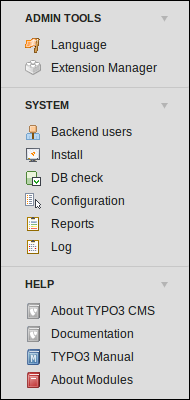
\includegraphics[width=0.35\linewidth]{Images/BackendChanges/AdminTools.png}
			\end{figure}
		\end{column}

	\end{columns}

\end{frame}

% ------------------------------------------------------------------------------
% Visual Appearance
% ------------------------------------------------------------------------------
% http://forge.typo3.org/issues/36017

\begin{frame}[fragile]
	\frametitle{Promene administratorskog dela}
	\framesubtitle{Vizualni prikaz}

	\begin{itemize}
		\item \texttt{<h1>}-naslovi u glavnom delu koriste TYPO3 font "Share"
	\end{itemize}

	\begin{figure}
		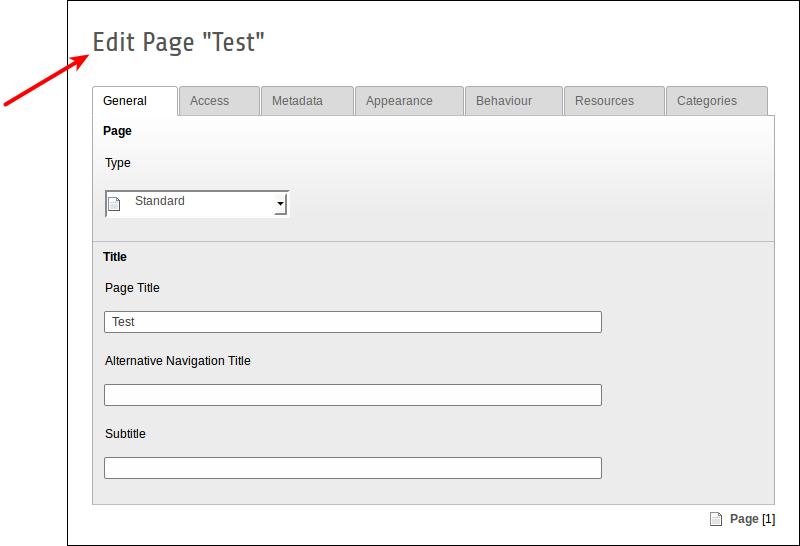
\includegraphics[width=0.6\linewidth]{Images/BackendChanges/ConsistantFont.png}
	\end{figure}

\end{frame}

% ------------------------------------------------------------------------------
% Visual Appearance
% ------------------------------------------------------------------------------
% http://forge.typo3.org/issues/41631

\begin{frame}[fragile]
	\frametitle{Promene administratorskog dela}
	\framesubtitle{Vizualni prikaz}

	\begin{itemize}
		\item Modul "Reports" ima novu ikonicu
	\end{itemize}

	\begin{figure}
		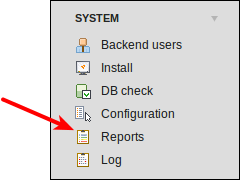
\includegraphics[width=0.35\linewidth]{Images/BackendChanges/ModuleReportsIcon.png}
	\end{figure}

\end{frame}

% ------------------------------------------------------------------------------
% Drag&Drop File Upload in Filelist (FAL)
% ------------------------------------------------------------------------------
% http://forge.typo3.org/issues/47005

\begin{frame}[fragile]
	\frametitle{Promene administratorskog dela}
	\framesubtitle{Drag\&Drop slanje fajlova (1)}

	\begin{itemize}
		\item HTML5 Drag\&Drop funkcionalnost za slanje fajlova implementirana u filelist

	\end{itemize}

	\begin{figure}
		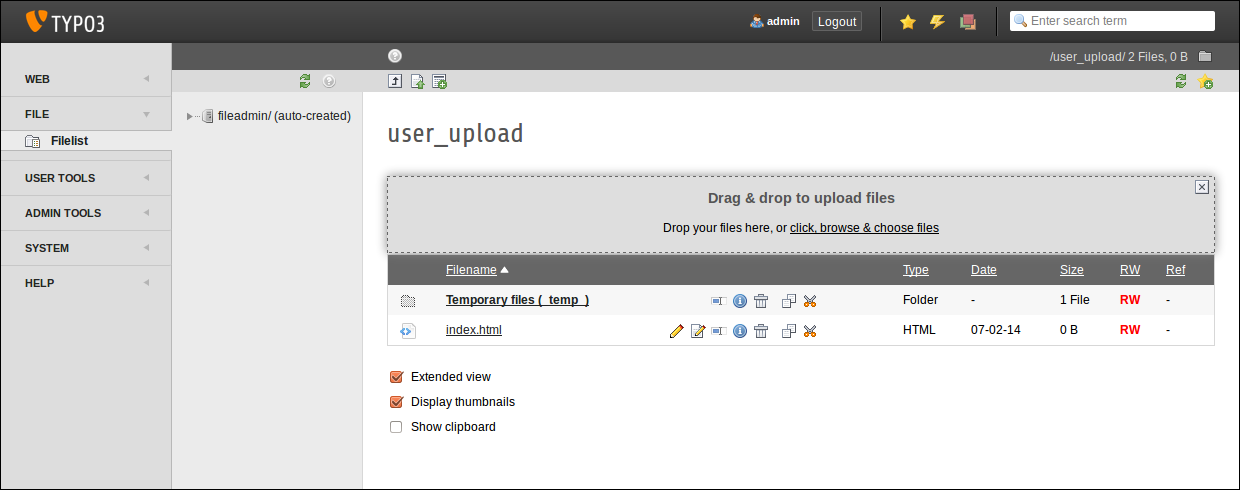
\includegraphics[width=0.95\linewidth]{Images/BackendChanges/DragDropFileUpload.png}
	\end{figure}

\end{frame}

% ------------------------------------------------------------------------------
% Drag&Drop File Upload Via Content Elements
% (slide added in March 2014)
% ------------------------------------------------------------------------------

\begin{frame}[fragile]
	\frametitle{Promene administratorskog dela}
	\framesubtitle{Drag\&Drop slanje fajlova (2)}

	\begin{itemize}
		\item ...i kod sadrzaja (dugme: "Select \& upload files")

	\end{itemize}

	\begin{figure}
		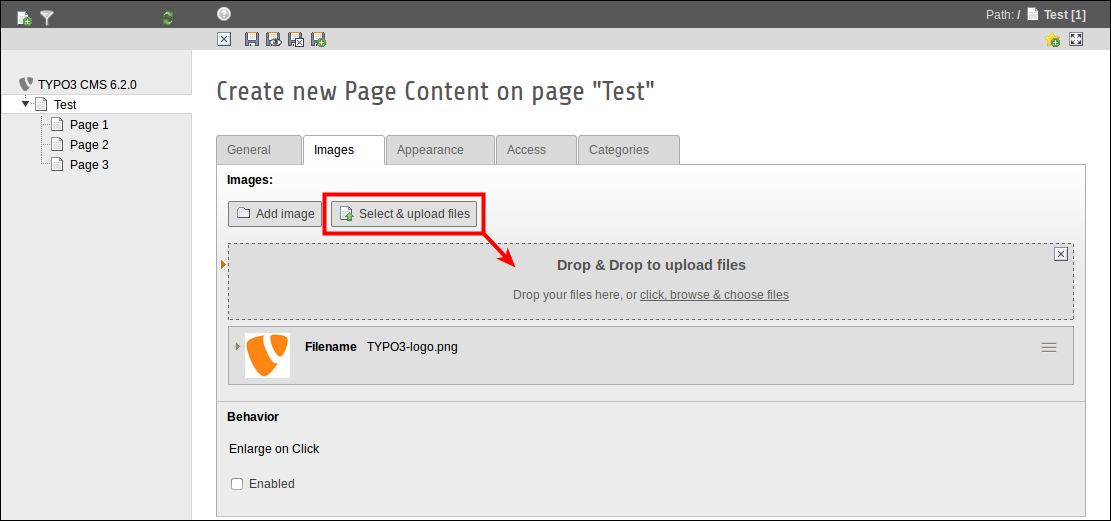
\includegraphics[width=0.95\linewidth]{Images/BackendChanges/SelectAndUploadFiles.png}
	\end{figure}

\end{frame}

% ------------------------------------------------------------------------------
% Backend Users
% ------------------------------------------------------------------------------
% http://forge.typo3.org/issues/43053

\begin{frame}[fragile]
	\frametitle{Promene administratorskog dela}
	\framesubtitle{Upotrebljivost: lista korisnika administratorskog dela}

	\begin{itemize}
		\item Korisnicko ime i pravo ime su prikazani (prva kolona u list view)
		\item Klikom na korisnicko ime (pravo ime) otvara se link za uredjivanje korisnickog naloga
		\item Dugme delete dodato je u list view

	\end{itemize}

	\begin{figure}
		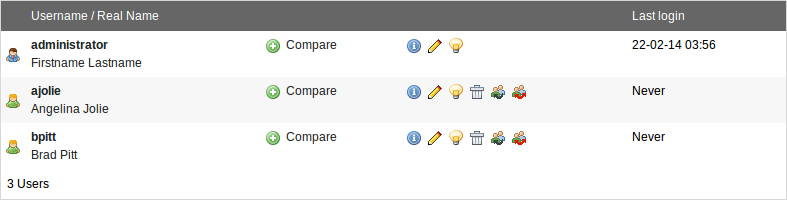
\includegraphics[width=0.95\linewidth]{Images/BackendChanges/BackendUserList.png}
	\end{figure}

\end{frame}

% ------------------------------------------------------------------------------
% Live Search
% ------------------------------------------------------------------------------
% http://forge.typo3.org/issues/35358

\begin{frame}[fragile]
	\frametitle{Promene administratorskog dela}
	\framesubtitle{Live Search}

	\begin{itemize}
		\item Tooltip pokazuje UID kao i PID u "livesearch"
		\item Kada se, nakon pretrage, uredjena forma zatvori, bice prikazan list view (a ne prazna strana)
	\end{itemize}

	\begin{figure}
		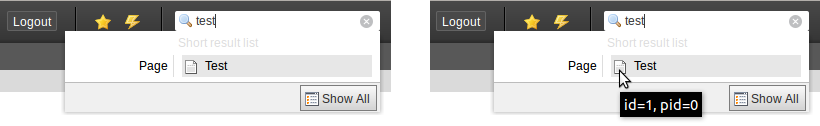
\includegraphics[width=0.8\linewidth]{Images/BackendChanges/LiveSearchTooltip.png}
	\end{figure}

\end{frame}

% ------------------------------------------------------------------------------
% Live Search
% ------------------------------------------------------------------------------

\begin{frame}[fragile]
	\frametitle{Promene administratorskog dela}
	\framesubtitle{Live Search}

	\begin{itemize}
		\item U TYPO3 < 6.2, za strane su uzimana u obzir samo polja iz baze \texttt{title} i \texttt{uid} 
		\item U TYPO3 >= 6.2, polje \texttt{alias} moze biti dodato u pretragu\newline
			(zahteva UserTSconfig: \texttt{options.pageTree.searchInAlias = 1})
	\end{itemize}

	\begin{figure}
		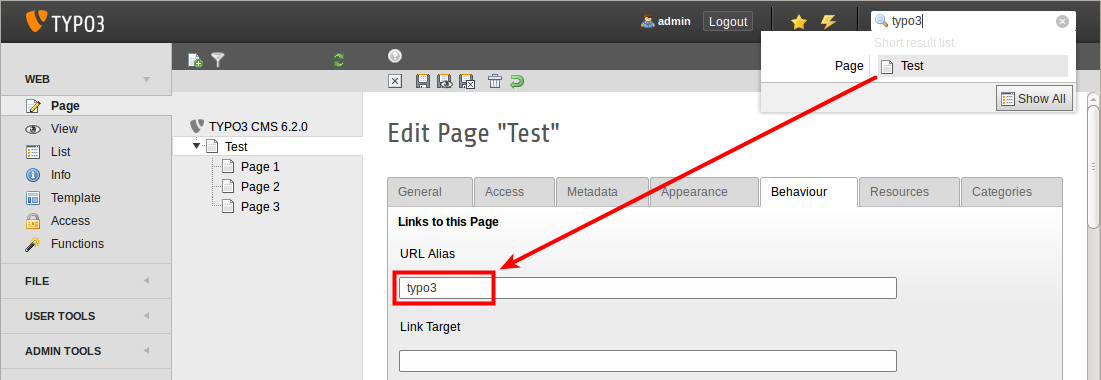
\includegraphics[width=0.95\linewidth]{Images/BackendChanges/LiveSearchInAlias.png}
	\end{figure}

\end{frame}

% ------------------------------------------------------------------------------
% File Abstraction Layer
% ------------------------------------------------------------------------------

\begin{frame}[fragile]
	\frametitle{Promene administratorskog dela}
	\framesubtitle{File Abstraction Layer}

	\begin{itemize}
		\item Naslov i ime fajla se prikazuju u zaglavlju FAL-a
	\end{itemize}

	\begin{figure}
		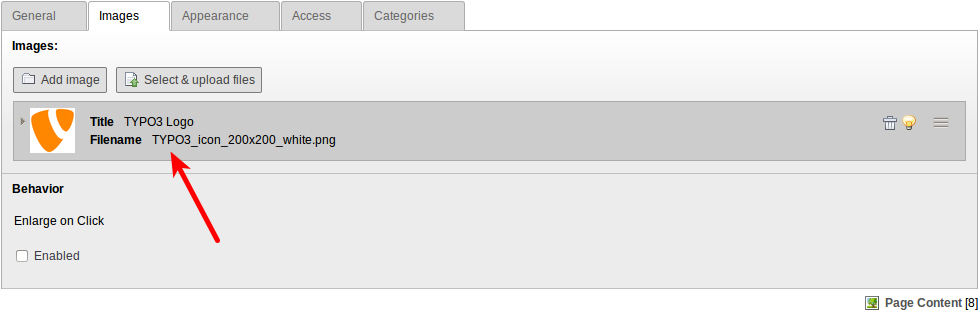
\includegraphics[width=0.95\linewidth]{Images/BackendChanges/FalTitleAndFilename.png}
	\end{figure}

\end{frame}

% ------------------------------------------------------------------------------
% File Abstraction Layer
% ------------------------------------------------------------------------------

\begin{frame}[fragile]
	\frametitle{Promene administratorskog dela}
	\framesubtitle{File Abstraction Layer (EXT:filemetadata)}

	\begin{itemize}
		\item Sistemsko prosirenje "filemetadata" dodaje kartice koje prikazuju meta podatke\newline
			\small(prosirenje se nalazi u instalaciji sistema, ali nije instalirano)\normalsize
	\end{itemize}

	\begin{figure}
		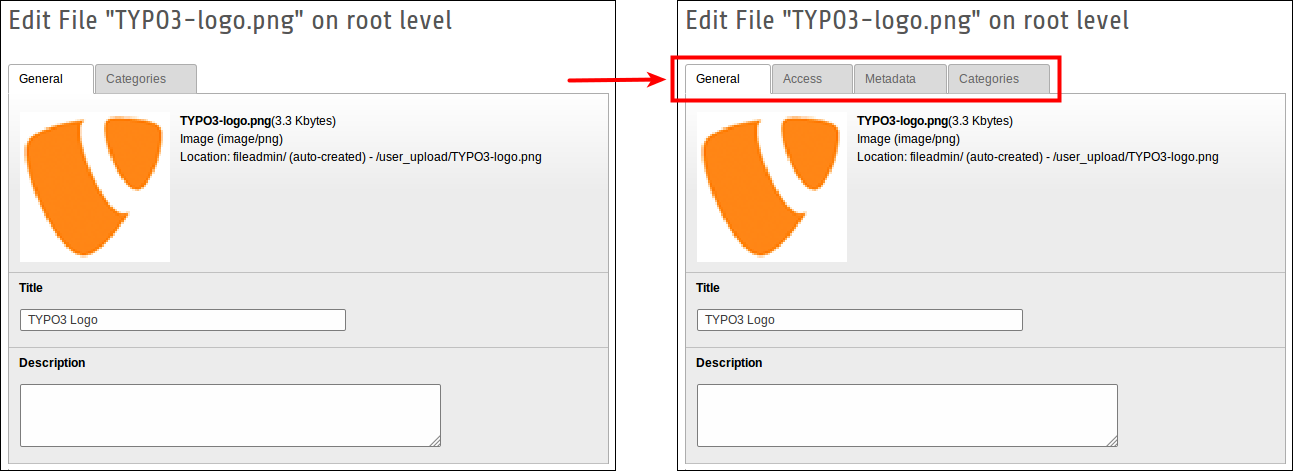
\includegraphics[width=0.95\linewidth]{Images/BackendChanges/FileMetaDataTabs.png}
	\end{figure}

\end{frame}

% ------------------------------------------------------------------------------
% File Abstraction Layer
% ------------------------------------------------------------------------------

\begin{frame}[fragile]
	\frametitle{Promene administratorskog dela}
	\framesubtitle{File Abstraction Layer (EXT:filemetadata)}

	\begin{figure}
		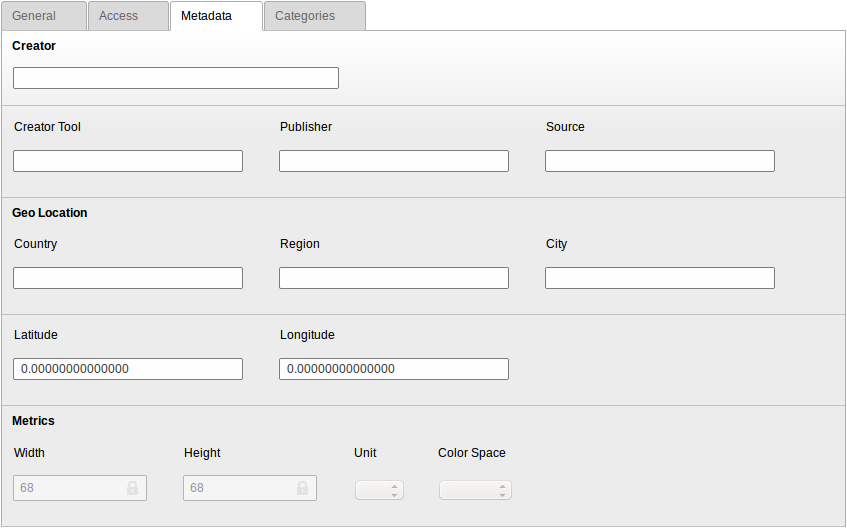
\includegraphics[width=0.8\linewidth]{Images/BackendChanges/FileMetaData.png}
	\end{figure}

\end{frame}

% ------------------------------------------------------------------------------
% File Abstraction Layer
% ------------------------------------------------------------------------------

\begin{frame}[fragile]
	\frametitle{Promene administratorskog dela}
	\framesubtitle{File Abstraction Layer}

	\begin{itemize}
		\item Sada je moguce je prevesti FAL meta podatke
	\end{itemize}

	\begin{figure}
		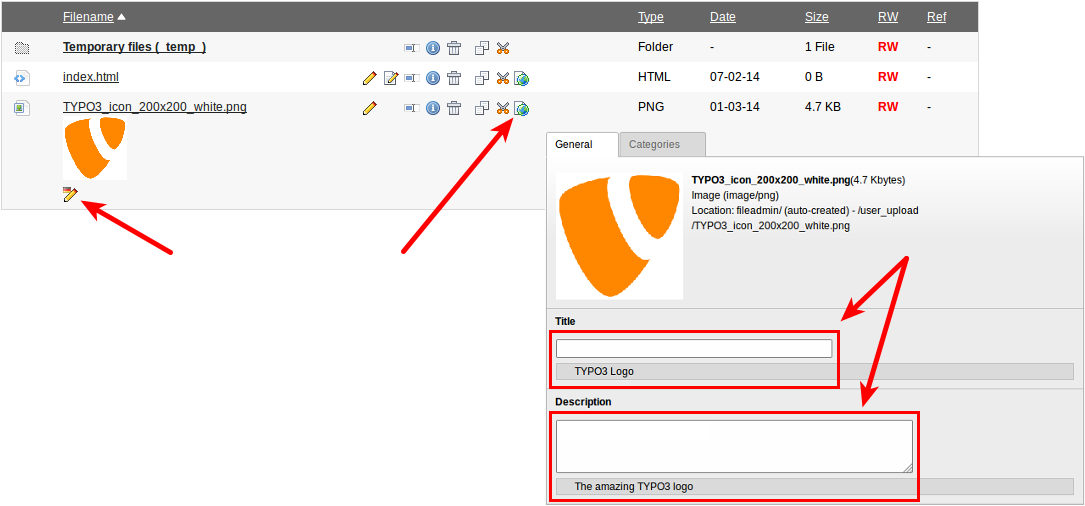
\includegraphics[width=0.95\linewidth]{Images/BackendChanges/FalTranslateMetaData.png}
	\end{figure}

\end{frame}

% ------------------------------------------------------------------------------
% Module: Documentation
% ------------------------------------------------------------------------------

\begin{frame}[fragile]
	\frametitle{Promene administratorskog dela}
	\framesubtitle{Modue: Documentation}

	\begin{columns}[T]

		\begin{column}{.5\textwidth}
			\begin{itemize}
				\item Modul "Documentation" dozvoljava administratorima da preuzimaju i pregledavaju uputstva
				\item Nova TYPO3 instalacija podrazumeva prisustvo ovog modula
				\item Funkcija "Manage Documentation" preuzima uputstva (pogledati ilustraciju)
				\item Preko Extension Manager-a moguce je ukljuciti ovaj modul kod azurirane TYPO3 instalacije
			\end{itemize}
		\end{column}

		\begin{column}{.5\textwidth}
			\begin{figure}\vspace*{-0.4cm}
				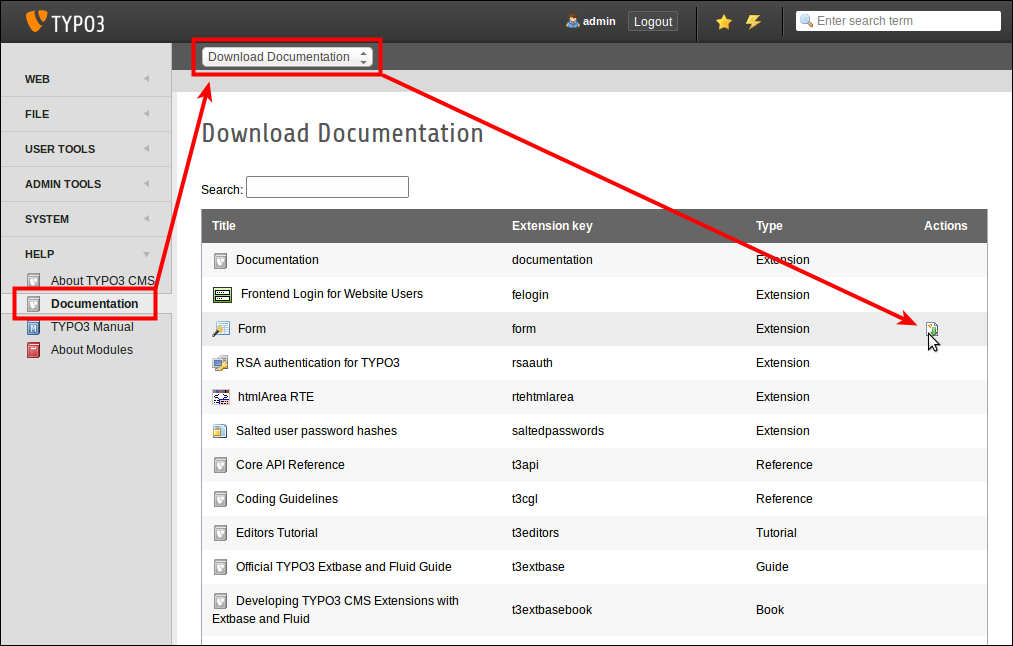
\includegraphics[width=1\linewidth]{Images/BackendChanges/DownloadDocumentation.png}
			\end{figure}
		\end{column}

	\end{columns}

\end{frame}

% ------------------------------------------------------------------------------
% Module: Documentation
% ------------------------------------------------------------------------------

\begin{frame}[fragile]
	\frametitle{Promene administratorskog dela}
	\framesubtitle{Modul: Documentation}

	\begin{itemize}
		\item Funkcija "Show Documentation" prikazuje preuzeta uputstva
	\end{itemize}

	\begin{figure}
		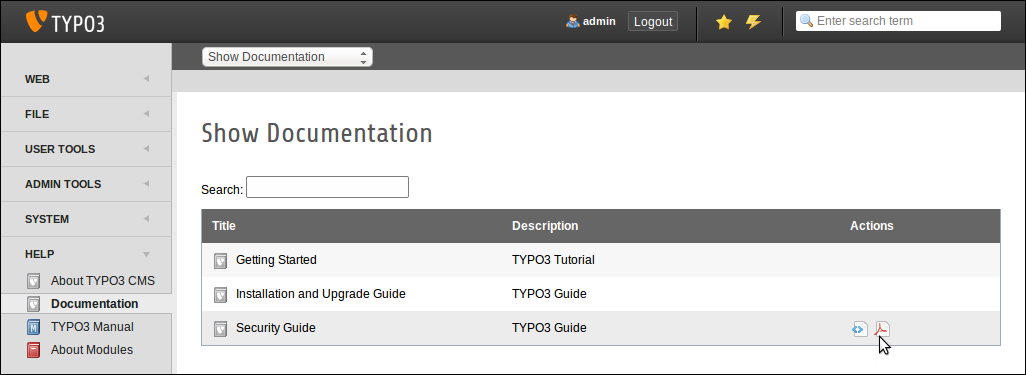
\includegraphics[width=0.95\linewidth]{Images/BackendChanges/ShowDocumentation.png}
	\end{figure}

\end{frame}

% ------------------------------------------------------------------------------
% Removed: TypoScript Help
% ------------------------------------------------------------------------------
% http://forge.typo3.org/issues/47931

\begin{frame}[fragile]
	\frametitle{Promene administratorskog dela}
	\framesubtitle{Uklonjeno: TypoScript Help}

 	\begin{itemize}
		\item EXT:tsconfig\_help ("TSconfig Quick Reference") uklonjeno\newline
			\small(zastarele informacije koje nisu menjane jos od TYPO3 CMS 4.1)
	\end{itemize}

	\begin{figure}
		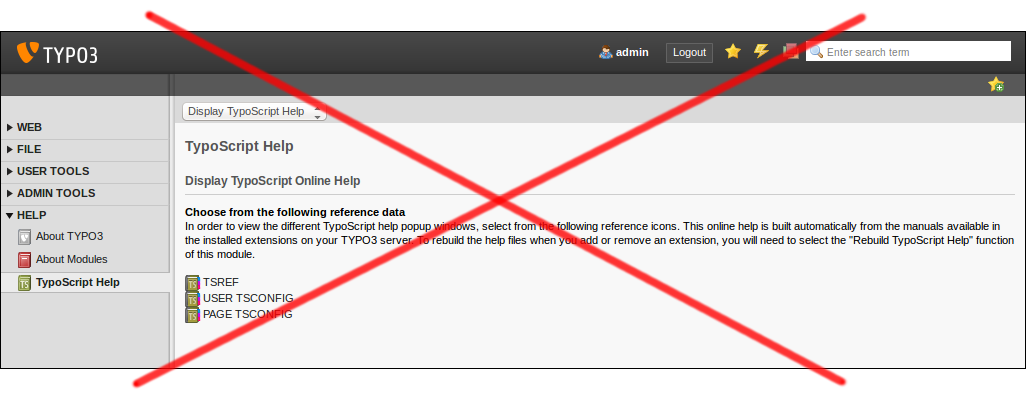
\includegraphics[width=0.95\linewidth]{Images/BackendChanges/TypoScriptHelpRemovedCrossed.png}
	\end{figure}

\end{frame}


% ------------------------------------------------------------------------------
% Scheduler
% ------------------------------------------------------------------------------

\begin{frame}[fragile]
	\frametitle{Promene administratorskog dela}
	\framesubtitle{Scheduler}

	\begin{itemize}
		\item Brisanje scheduler task-a pregledu za izmenu\newline
			\small(U TYPO3 < 6.2, opcija za brisanje bila je dostupna samo u list view)\normalsize
	\end{itemize}

	\begin{figure}
		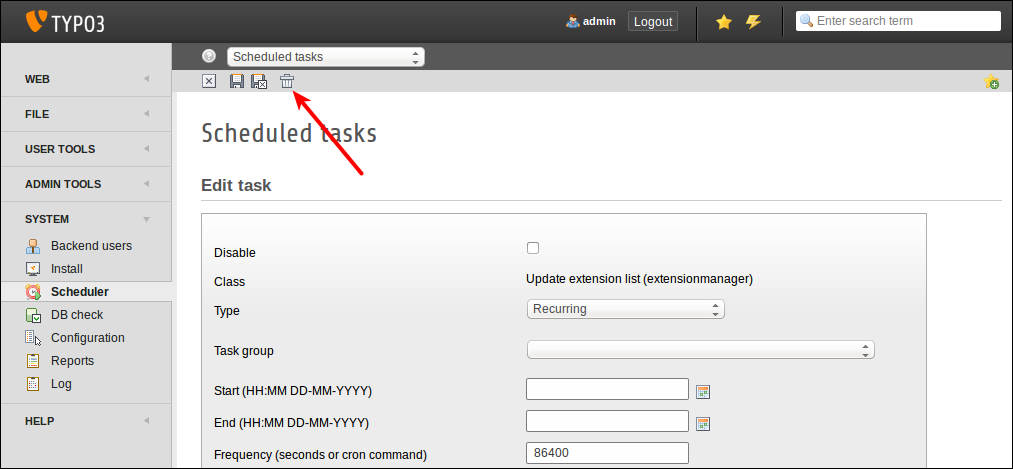
\includegraphics[width=0.95\linewidth]{Images/BackendChanges/DeleteSchedulerTaskInEditView.png}
	\end{figure}

\end{frame}

% ------------------------------------------------------------------------------
% Scheduler
% ------------------------------------------------------------------------------

\begin{frame}[fragile]
	\frametitle{Promene administratorskog dela}
	\framesubtitle{Scheduler}

	\begin{itemize}
		\item Scheduler zadaci mogu sadrzati opise koji se prikazuju kao podnaslovi u list pregledu, ili kao tultipovi (pogledati sledeci slajd)
	\end{itemize}

	\begin{figure}
		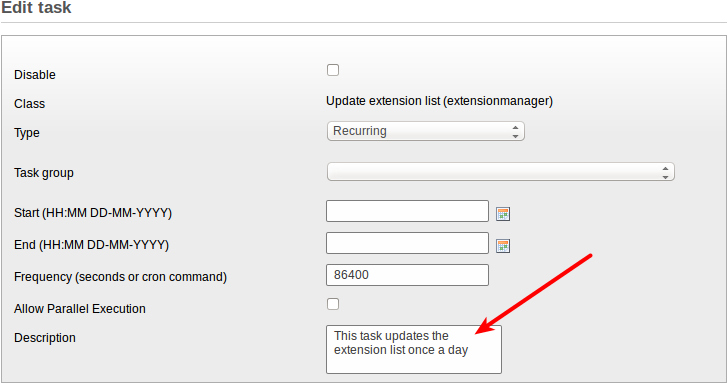
\includegraphics[width=0.7\linewidth]{Images/BackendChanges/SchedulerTaskDescription.png}
	\end{figure}

\end{frame}

% ------------------------------------------------------------------------------
% Scheduler
% ------------------------------------------------------------------------------

\begin{frame}[fragile]
	\frametitle{Promene administratorskog dela}
	\framesubtitle{Scheduler}

	\begin{itemize}
		\item Opis zadatka kao podnaslov\newline
			\small(ova opcija mora biti aktivirana u konfiguraciji prosirenja)\normalsize
	\end{itemize}

	\begin{figure}
		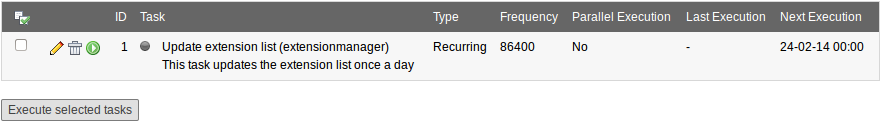
\includegraphics[width=0.95\linewidth]{Images/BackendChanges/SchedulerTaskDescriptionAsSubheader.png}
	\end{figure}

	\begin{itemize}
		\item Opis zadatka se prikazuje kao tultip 
		("hover")
	\end{itemize}

	\begin{figure}
		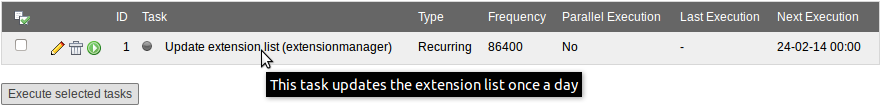
\includegraphics[width=0.95\linewidth]{Images/BackendChanges/SchedulerTaskDescriptionAsTooltip.png}
	\end{figure}

\end{frame}

% ------------------------------------------------------------------------------
% Scheduler
% ------------------------------------------------------------------------------

\begin{frame}[fragile]
	\frametitle{Promene administratorskog dela}
	\framesubtitle{Scheduler}

	\begin{itemize}
		\item Sada je moguce grupisanje scheduler task-ova
		\item Dodati "scheduler task group" rut strani (UID: 0)\newline
			i izabrati grupu
	\end{itemize}

	\begin{figure}
		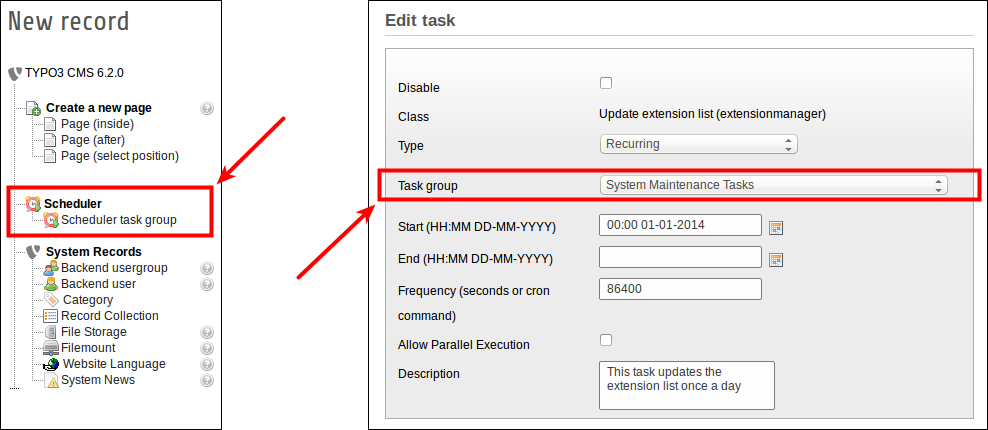
\includegraphics[width=0.85\linewidth]{Images/BackendChanges/SchedulerTaskGroup.png}
	\end{figure}

\end{frame}

% ------------------------------------------------------------------------------
% System Extension: Form
% ------------------------------------------------------------------------------
% http://forge.typo3.org/issues/38094

\begin{frame}[fragile]
	\frametitle{Promene administratorskog dela}
	\framesubtitle{Sistemsko prosirenje: Form}

	\begin{columns}[T]

		\begin{column}{.5\textwidth}
			\begin{itemize}
				\item Novi post-processor za cObject FORM: \textbf{redirect}\newline
					(redirekcija nakon postavljanja forme)
				\item Vrednost parsira \texttt{typolink} (TypoScript funkcija),\newline
					sto znaci da vrednost moze biti ID strane ili URL
			\end{itemize}
		\end{column}

		\begin{column}{.5\textwidth}
			\begin{figure}\vspace*{-0.4cm}
				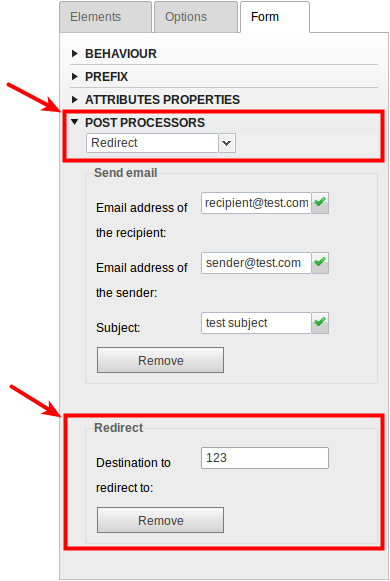
\includegraphics[width=0.65\linewidth]{Images/BackendChanges/FormRedirectPostProcessor.png}
			\end{figure}
		\end{column}

	\end{columns}

\end{frame}

% ------------------------------------------------------------------------------
% Module: List
% ------------------------------------------------------------------------------
% http://forge.typo3.org/issues/49810

\begin{frame}[fragile]
	\frametitle{Promene administratorskog dela}
	\framesubtitle{List Modul}

	\begin{itemize}
		\item Dodatne kolone "UID" i "PID" kod list view-a za uredjivace
	\end{itemize}

	\begin{figure}
		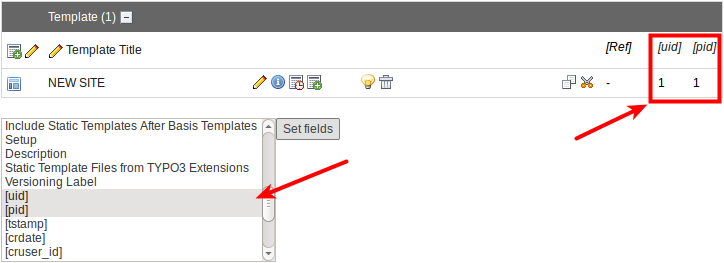
\includegraphics[width=0.95\linewidth]{Images/BackendChanges/AdditionalColumnsInListModule.png}
	\end{figure}

\end{frame}

% ------------------------------------------------------------------------------
% File Abstraction Layer
% ------------------------------------------------------------------------------
% http://forge.typo3.org/issues/50827
% http://forge.typo3.org/issues/51097

\begin{frame}[fragile]
	\frametitle{Promene administratorskog dela}
	\framesubtitle{File Abstraction Layer}

	\begin{itemize}
		\item Ako indexer uoci da neki fajl nedostaje priikazuje se poruka i upisuje se u bazi podataka da fajl nedostaje
		\item Modul "Reports" takodje prikazuje ovaj problem
		\item Kada se fajl vrati, poruka i zapis u bazi podataka se brisu
	\end{itemize}

	\begin{columns}[T]

		\begin{column}{.5\textwidth}
			\begin{figure}
				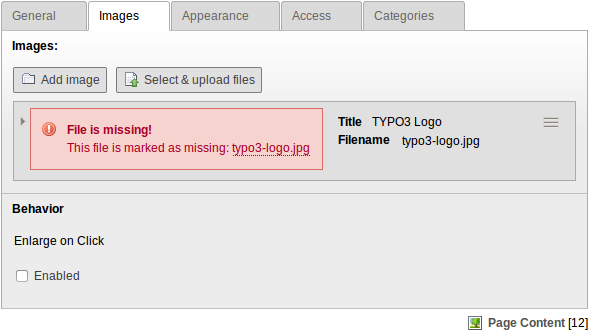
\includegraphics[width=0.95\linewidth]{Images/BackendChanges/FalMissingFileContentElement.png}
			\end{figure}
		\end{column}

		\begin{column}{.5\textwidth}
			\begin{figure}
				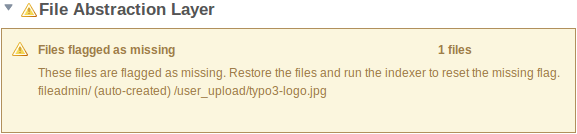
\includegraphics[width=0.95\linewidth]{Images/BackendChanges/FalMissingFileReportsModule.png}
			\end{figure}
		\end{column}

	\end{columns}

\end{frame}

% ------------------------------------------------------------------------------
% Menu/Sitemap: Category-based Menus
% ------------------------------------------------------------------------------
% http://forge.typo3.org/issues/51161

\begin{frame}[fragile]
	\frametitle{Promene administratorskog dela}
	\framesubtitle{Meniji kategorija (1)}

	\begin{itemize}
		\item Elemenat sadrzaja "Menu/Sitemap" moze da napravi meni u zavisnosti od kategorija
	\end{itemize}

	\begin{figure}
		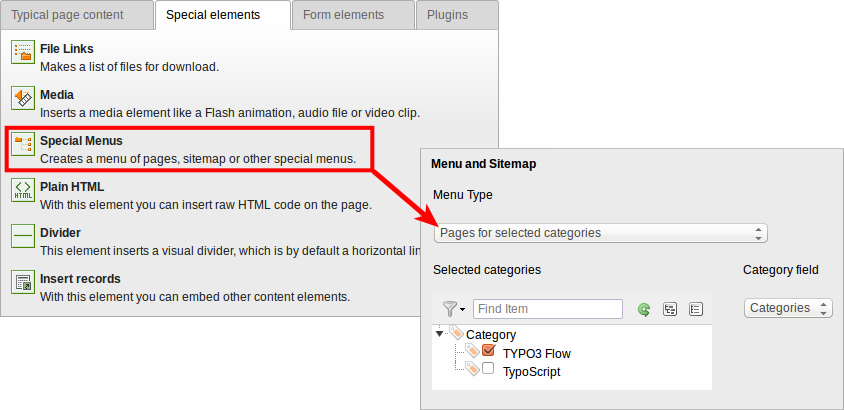
\includegraphics[width=0.8\linewidth]{Images/BackendChanges/CategoryBasedMenus.png}
	\end{figure}

\end{frame}

% ------------------------------------------------------------------------------
% Menu/Sitemap: Category-based Menus
% (slide added in March 2014)
% ------------------------------------------------------------------------------

\begin{frame}[fragile]
	\frametitle{Promene administratorskog dela}
	\framesubtitle{Meniji kategorija (2)}

	\begin{itemize}
		\item Novi tip menija: "\underline{Elemenat sadrzaja} za selektovane kategorije"
	\end{itemize}

	\begin{figure}
		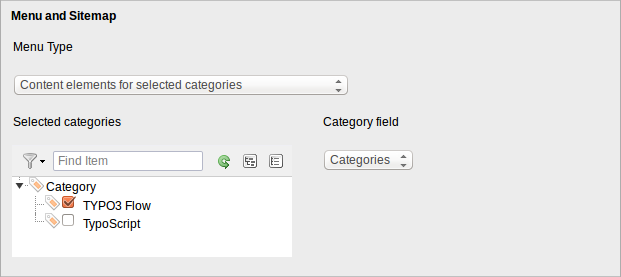
\includegraphics[width=0.6\linewidth]{Images/BackendChanges/ContentElementsForSelectedCategories.png}
	\end{figure}

\end{frame}

% ------------------------------------------------------------------------------
% Sorting Categories
% ------------------------------------------------------------------------------
% http://forge.typo3.org/issues/51590

\begin{frame}[fragile]
	\frametitle{Promene administratorskog dela}
	\framesubtitle{Sortiranje kategorija}

 	\begin{itemize}
		\item Sada kategorije mogu biti sortirane\newline
			\small(u TYPO3 < 6.2, kategorije su uvek sortirane abecednim redosledom)\normalsize
	\end{itemize}

	\begin{figure}
		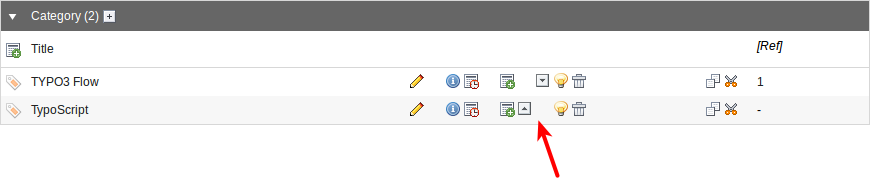
\includegraphics[width=0.95\linewidth]{Images/BackendChanges/CategorySorting.png}
	\end{figure}

\end{frame}

% ------------------------------------------------------------------------------
% Category Visibility
% ------------------------------------------------------------------------------
% http://forge.typo3.org/issues/52718

\begin{frame}[fragile]
	\frametitle{Promene administratorskog dela}
	\framesubtitle{Vidljivost kategorija}

 	\begin{itemize}
		\item Vidljivost kategorija moze biti zabranjena za uredjivace i grupe uredjivaca
	\end{itemize}

	\begin{figure}
		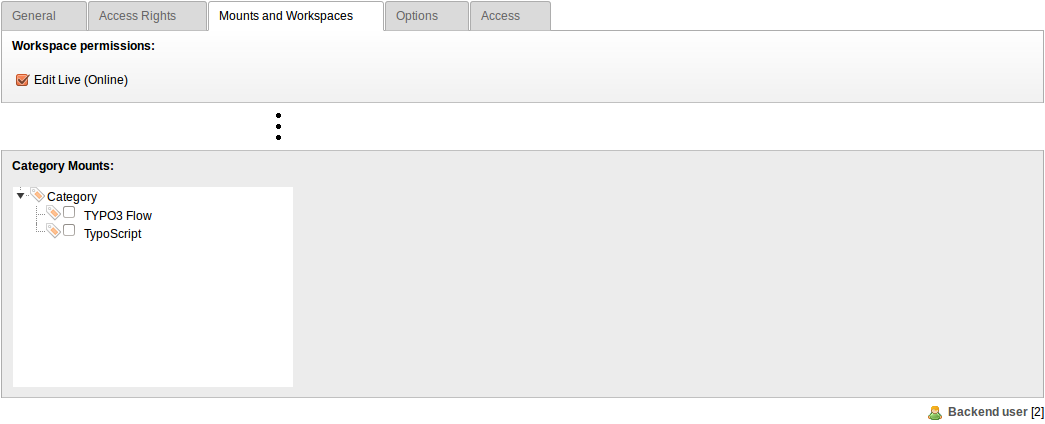
\includegraphics[width=0.95\linewidth]{Images/BackendChanges/CategoryVisibility.png}
	\end{figure}

\end{frame}

% ------------------------------------------------------------------------------
% "New Content" icon always visible
% ------------------------------------------------------------------------------
% http://forge.typo3.org/issues/48938
% http://forge.typo3.org/issues/51480

\begin{frame}[fragile]
	\frametitle{Promene administratorskog dela}
	\framesubtitle{Korisnost}

 	\begin{itemize}
		\item Ikonica "new content" je uvek vidljiva ako je kolona prazna\newline
			\small(ovo pomaze uredjivacima da razumeju sta mogu da urade)\normalsize
	\end{itemize}

	\begin{figure}
		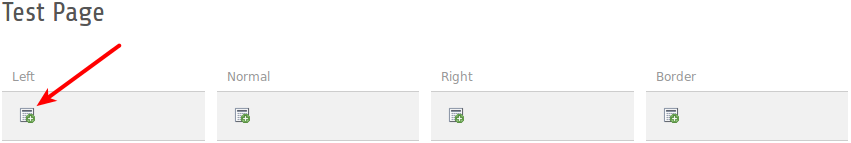
\includegraphics[width=0.95\linewidth]{Images/BackendChanges/NewContentIconAlwaysVisible.png}
	\end{figure}

\end{frame}

% ------------------------------------------------------------------------------
% Module "Functions": Hide In Menus
% ------------------------------------------------------------------------------
% http://forge.typo3.org/issues/51017

\begin{frame}[fragile]
	\frametitle{Promene administratorskog dela}
	\framesubtitle{Functions}

 	\begin{itemize}
		\item Kada se kreira vise strana odjednom u modulu "functions", novi cek boks omogucava uredjivacima da sakriju ove strane u meniju\newline
			\small(very useful, when creating a number of pages at a time)\normalsize
	\end{itemize}

	\begin{figure}
		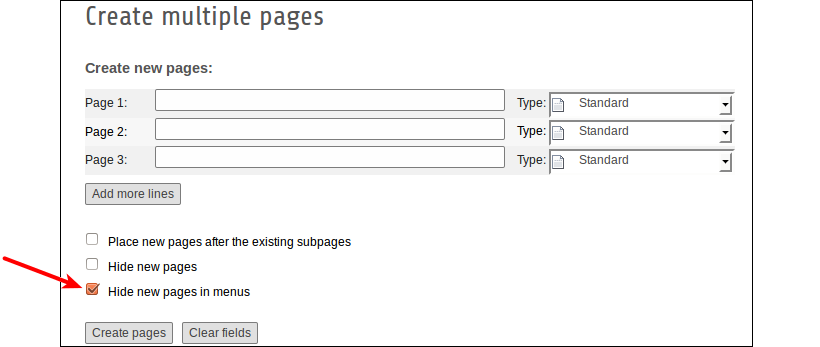
\includegraphics[width=0.85\linewidth]{Images/BackendChanges/CreateMultiplePagesHideInMenu.png}
	\end{figure}

\end{frame}

% ------------------------------------------------------------------------------
% Extension Manager: Upload Extensions
% ------------------------------------------------------------------------------
% http://forge.typo3.org/issues/51776
% http://forge.typo3.org/issues/51437

\begin{frame}[fragile]
	\frametitle{Promene administratorskog dela}
	\framesubtitle{Extension Manager}

 	\begin{itemize}
		\item Snimanje prosirenja pomocu funkcije "Get Extensions"
	\end{itemize}

	\begin{figure}
		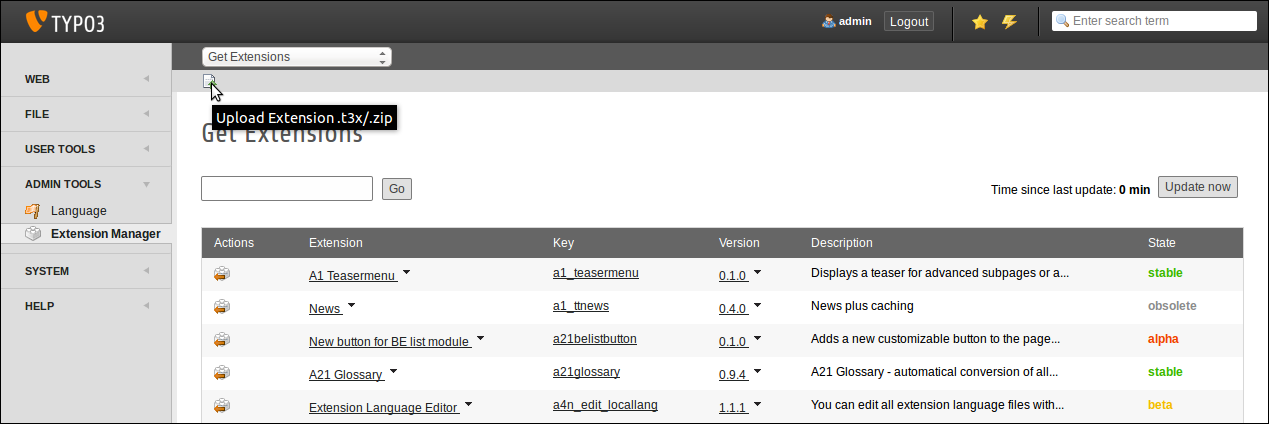
\includegraphics[width=0.95\linewidth]{Images/BackendChanges/UploadExtension.png}
	\end{figure}

\end{frame}

% ------------------------------------------------------------------------------
% Recycler
% ------------------------------------------------------------------------------
% http://forge.typo3.org/issues/52324

\begin{frame}[fragile]
	\frametitle{Promene administratorskog dela}
	\framesubtitle{Recycler}

 	\begin{itemize}
		\item Zapisi iz Recycler-a mogu biti sortirani po datumu\newline
			\small(Ovo pomaze uredjivacima da odluce da li da povrate odredjeni fajl ili ne)\normalsize
	\end{itemize}

	\begin{figure}
		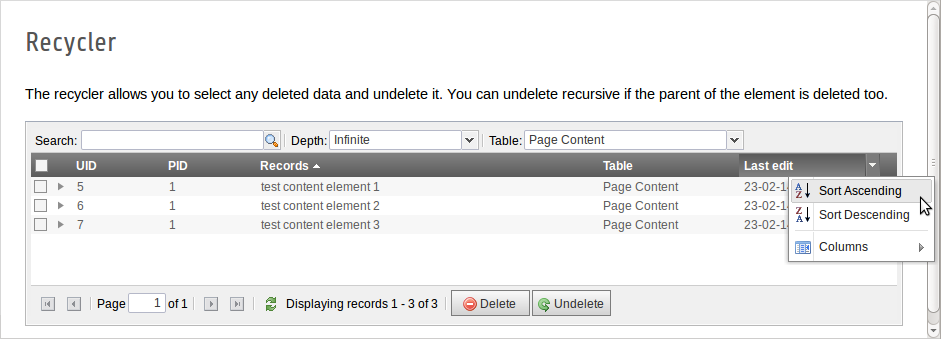
\includegraphics[width=0.95\linewidth]{Images/BackendChanges/RecyclerSortRecord.png}
	\end{figure}

\end{frame}

% ------------------------------------------------------------------------------
% File/Directory Permissions
% ------------------------------------------------------------------------------

\begin{frame}[fragile]
	\frametitle{Promene administratorskog dela}
	\framesubtitle{Permisije za fajlove i direktorijume}

 	\begin{itemize}
		\item Vise opcija kod postavljanja permisija fajlova i direktorijuma za uredjivace i grupe uredjivaca
			\begingroup\color{typo3red}\textbf{(1)}\endgroup
		\item Ovo je moguce od TYPO3 6.0, ali samo preko UserTSconfig
			\begingroup\color{typo3red}\textbf{(2)}\endgroup
	\end{itemize}

	\begin{figure}
		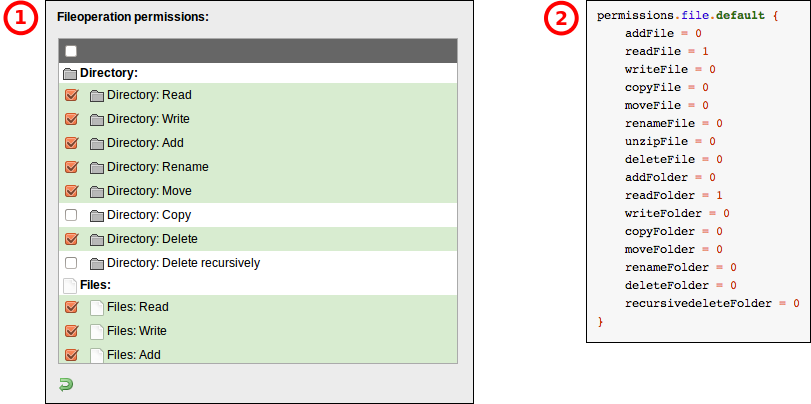
\includegraphics[width=0.75\linewidth]{Images/BackendChanges/FileAndDirectoryPermissions.png}
	\end{figure}

\end{frame}

% ------------------------------------------------------------------------------
% OpenID
% ------------------------------------------------------------------------------

\begin{frame}[fragile]
	\frametitle{Promene administratorskog dela}
	\framesubtitle{OpenID (1)}

 	\begin{itemize}
		\item OpenID za autentifikaciju uredjivaca moze biti postavljen preko carobnjaka
		\item EXT:openid (sistemsko prosirenje) je neophodno za ovo
	\end{itemize}

	\begin{figure}
		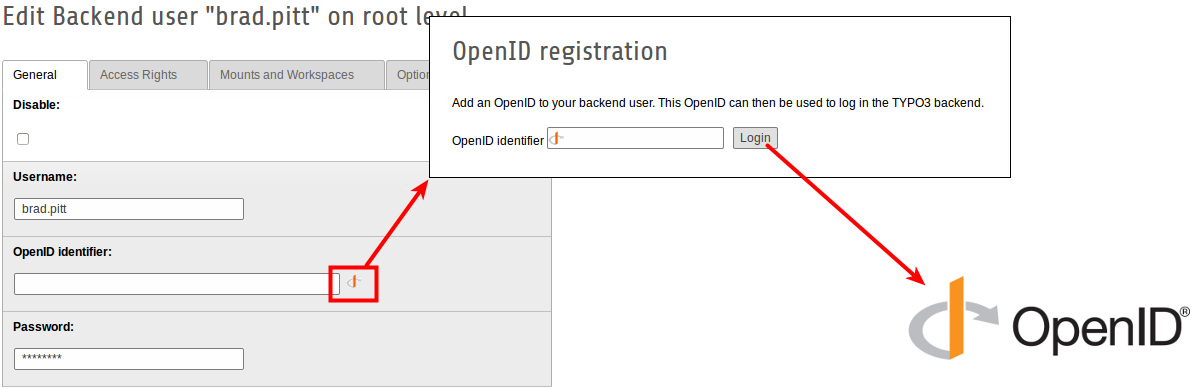
\includegraphics[width=0.95\linewidth]{Images/BackendChanges/OpenIdWizard.png}
	\end{figure}

\end{frame}

% ------------------------------------------------------------------------------
% OpenID
% ------------------------------------------------------------------------------

\begin{frame}[fragile]
	\frametitle{Promene administratorskog dela}
	\framesubtitle{OpenID (2)}

 	\begin{itemize}
		\item OpenID za autentifikaciju uredjivaca moze biti postavljen preko carobnjaka
		\item EXT:openid (sistemsko prosirenje) je neophodno za ovo
	\end{itemize}

	\begin{figure}
		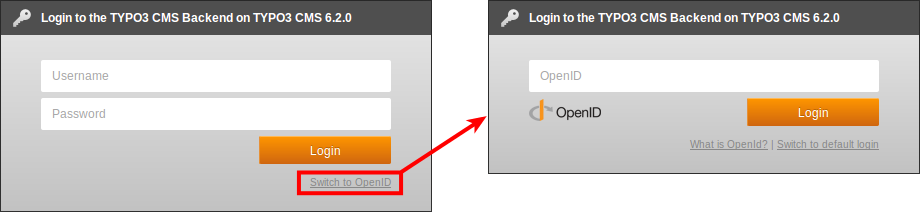
\includegraphics[width=0.8\linewidth]{Images/BackendChanges/OpenIdLogin.png}
	\end{figure}

 	\begin{itemize}
		\item Further details about OpenID:\newline
			\small\url{http://openid.net}\normalsize
	\end{itemize}

\end{frame}

% ------------------------------------------------------------------------------
% Workspaces 
% ------------------------------------------------------------------------------
% http://forge.typo3.org/issues/50223
% http://forge.typo3.org/issues/50224

\begin{frame}[fragile]
	\frametitle{Promene administratorskog dela}
	\framesubtitle{Workspaces}

 	\begin{itemize}
		\item Uredjivaci mogu da definisu koga da obaveste, bez ogranicenja sisatema
		\item Tab "All" je od sada vidljiv \underline{svim} korisnicima
	\end{itemize}

	\begin{figure}
		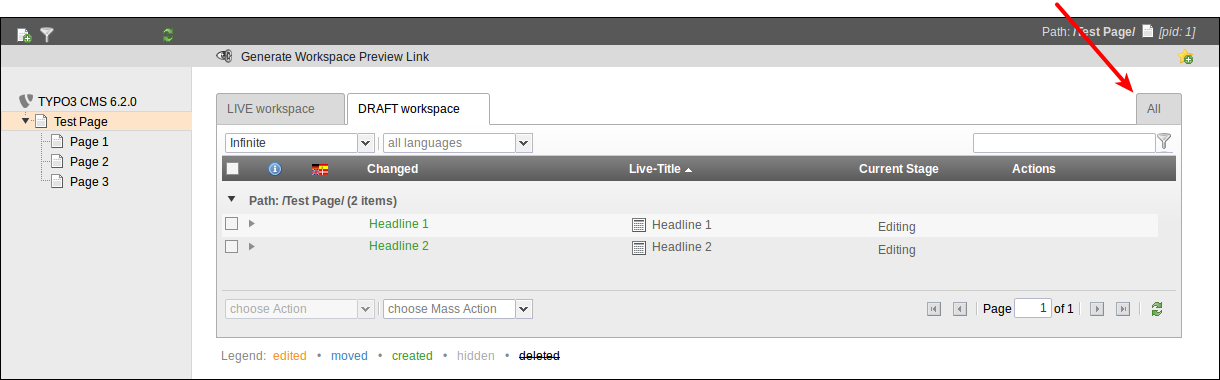
\includegraphics[width=0.95\linewidth]{Images/BackendChanges/WorkspacesTabAll.png}
	\end{figure}

\end{frame}

% ------------------------------------------------------------------------------